\documentclass[letter,12pt]{article}
\usepackage[letterpaper,right=1in,left=1in,top=1in,bottom=1in]{geometry}
\usepackage{setspace}

\usepackage[utf8]{inputenc}   % allows input of special characters from keyboard (input encoding)
\usepackage[T1]{fontenc}      % what fonts to use when printing characters       (output encoding)
\usepackage{amsmath}          % facilitates writing math formulas and improves the typographical quality of their output
\usepackage[hyphens]{url}     % adds line breaks to long urls
\usepackage[pdftex]{graphicx} % enhanced support for graphics
\usepackage{tikz}             % Easier syntax to draw pgf files (invokes pgf automatically)
\usetikzlibrary{arrows}

\usepackage{mathptmx}           % set font type to Times
\usepackage[scaled=.90]{helvet} % set font type to Times (Helvetica for some special characters)
\usepackage{courier}            % set font type to Times (Courier for other special characters)

\usepackage[longnamesfirst, sort]{natbib}\bibpunct[]{(}{)}{,}{a}{}{;} % handles biblio and references 

\usepackage{rotating}         % sideway tables and figures that take a full page
\usepackage{caption}          % allows multipage figures and tables with same caption (\ContinuedFloat)

\usepackage{dcolumn}          % needed for apsrtable and stargazer tables from R to compile
\usepackage{arydshln}         % dashed lines in tables (hdashline, cdashline{3-4}, 
                              %see http://tex.stackexchange.com/questions/20140/can-a-table-include-a-horizontal-dashed-line)
                              % must be loaded AFTER dcolumn, 
                              %see http://tex.stackexchange.com/questions/12672/which-tabular-packages-do-which-tasks-and-which-packages-conflict


\newcommand{\mc}{\multicolumn}

%% TO ADD NOTES IN TEXT, PUT % BEFORE THE ONE YOU WANT DISABLED
\usepackage[disable]{todonotes}                            % no show
%\usepackage[colorinlistoftodos, textsize=small]{todonotes} % show notes
\newcommand{\emm}[1]{\todo[color=red!15, inline]{\textbf{Eric:} #1}}

%% \usepackage{xr} % allows cross-ref to other file
%% \externaldocument{urge15appendix}

%% %for submission: sends figs, tables, and footnotes to last pages
%% \RequirePackage[nomarkers,nolists]{endfloat}     % sends tables and figures to the end
%% \RequirePackage{endnotes}                        % turns fn into endnotes; place \listofendnotes where you want 
%%                                                  %the endnotes to appear (it must be after the last endnote).
%% \let\footnote=\endnote
%% \newcommand{\listofendnotes}{
%%    \begingroup
%%    \parindent 0pt
%%    \parskip 2ex
%%    \def\enotesize{\normalsize}
%%    \theendnotes
%%    \endgroup
%% }

%% % for submission: drop page numbers when producing title page
%% \pagenumbering{gobble} % Remove page numbers (and reset to 1)
%% \pagenumbering{arabic}% Arabic page numbers (and reset to 1)


\setcitestyle{citesep={;}}

\begin{document}

\title{Incumbency advantage upon removal of single-term limits: Mexican municipal elections}
\author{Eric Magar \\ ITAM, Mexico City
}
\date{\today}
\maketitle

% \newpage

\begin{abstract}
\noindent En route
%% \newline
%% \newline
%% \textbf{Keywords}: Separation of Powers, Urgency Prerrogatives, Fast Track Authority, Legislative Process, Latin America, Chile
\end{abstract}

% \newpage

%\doublespacing

\section{Introduction}

\noindent En route

\section{A hypothesis perhaps}

\begin{figure}
  \centering
    \caption{The president rules game}\label{F:game}
    \tikzstyle{mid}=[circle,draw]
    \begin{tikzpicture}
      \node[mid] at (1.5,-0.25) (c) {\emph{C}};
      \node[mid] at (4,1) (p) {\emph{P}};
      \node[mid] at (6.5,-0.25) (f) {\emph{F}};
      \node at (4,-1.5) (ce) {$q$};
      \node at (6.5,2.25) (pe1) {$x_F$};
      \node at (9,1) (fe1) {$x_C$};
      \node at (9,-1.5) (fe2) {$q$};
      \path[-] (c) edge node [above, sloped] {\footnotesize{report}} (p)
               (p) edge node [above, sloped] {\footnotesize{fast}} (f)
                   edge node [below, sloped] {\footnotesize{track}} (f);
      \path[] (c) edge node [below, sloped] {\footnotesize{$x_C$}} (p);
      \path[-o] (c) edge node [below, sloped] {\footnotesize{not}} (ce)
                (p) edge node [above, sloped] {\footnotesize{standard}} (pe1)
                (f) edge node [above, sloped] {\footnotesize{accept}} (fe1)
                    edge node [below, sloped] {\footnotesize{reject}} (fe2);
      \path[-o] (p) edge node [below, sloped] {\footnotesize{considerat.}} (pe1);
    \end{tikzpicture}
\end{figure}

\begin{description}
  \item [Hypothesis 1:] Presidents are more likely to fast-track bills when the committee chair with jurisdiction over the bill  belongs to the president's party than otherwise.
\end{description}

\section{Regression model}



\section{Discussion}

\begin{figure}
  \centering
    \caption{Population-weigthed altitude deviations in municipalities}\label{F:avgMg}
    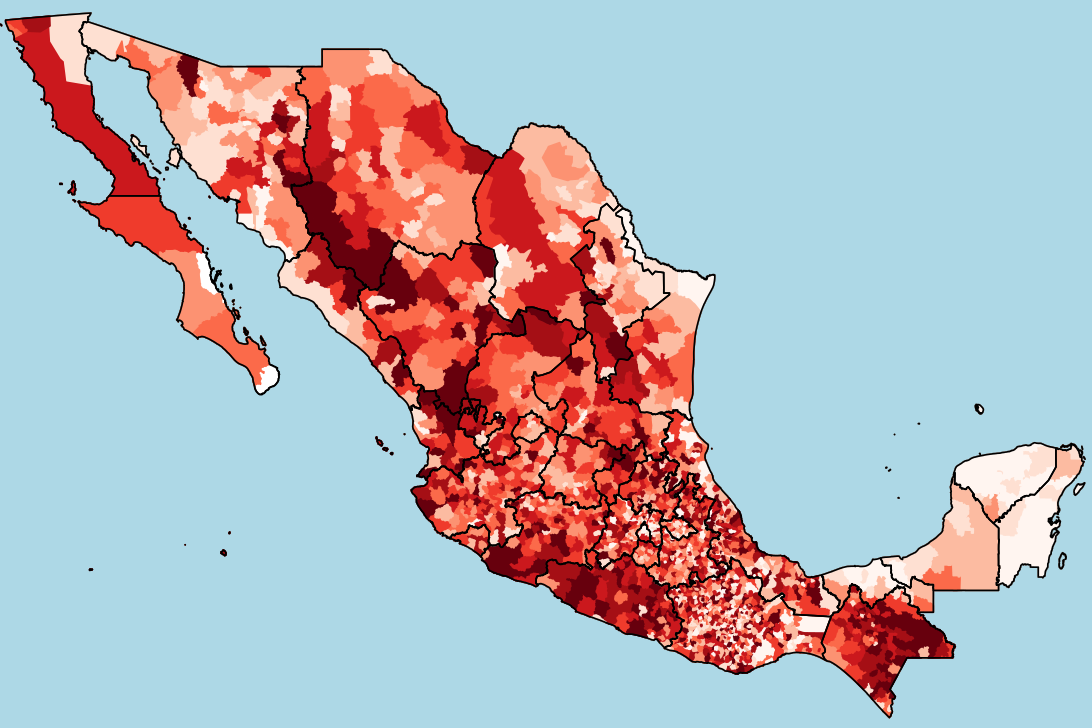
\includegraphics[width=.8\columnwidth]{../graph/map.png}
\end{figure}


\section*{Acknowledgements}
The author received financial support from the Asociaci\'on Mexicana de Cultura \textsc{a.c.}\ and \textsc{conacyt}'s Sistema Nacional de Investigadores. He is responsible for mistakes and shortcomings in the study.

%% \listofendnotes

\bibliographystyle{apsr}
\bibliography{../bib/magar}

\end{document}

